\subsection{Herstellung von polymer optischen Wellenleitern}
\label{subsec:pofherstellungsverfahren}

\subsubsection{Herstellung einer SI-POF mittels Extrusion}

Für die Herstellung eines polymeren Wellenleiters mit Stufenindexprofil eignet
sich die kontinuierliche Extrusion (siehe \autoref{fig:pofsispinn}). Dabei
werden die Monomere samt Radikalstarter und Additiven in ein geheiztes
Polymerisationsgefäß (\textit{heating unit}) gegeben. Nachdem der Polymeranteil
in der Reaktionskammer hoch genug ist, werden die Polymere in den Extruder
gepumpt und von diesem in eine Spinndüse gedrückt. In der Spinndüse wird der
Kern der polymer optischen Faser geformt und mit einem Mantel umgeben, der aus
einem Extruder mit dem Mantelmaterial (\textit{cladding material}) kommt. Der
Faden wird dann in einer \textit{blow box} gekühlt, gedehnt
(\textit{stretching}) und aufgerollt (\textit{take-up}). Dieses Verfahren ist
für die Massenproduktion geeignet. Da kein vorgefertigtes Granulat verwendet
wird, hat der Kern eine hohe Reinheit. Ein Nachteil dieses Verfahren sind jedoch
die hohen Kosten.

\begin{figure}[h]
    \begin{center}
        \begin{minipage}[t]{\textwidth}
            \begin{center}
                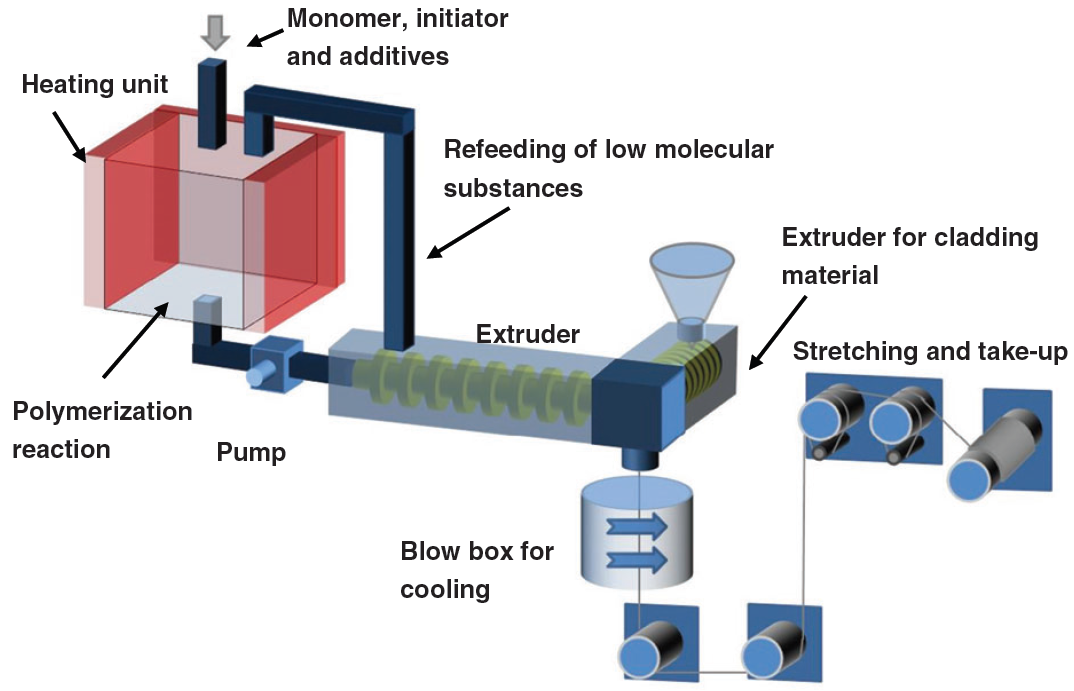
\includegraphics[height=0.25\textheight]{Bilder/Optische_Wellenleiter_Die_Polymer_Optische_Faser/Herstellung/pofsispinn.png}
                \caption[kontinuirliche Extrusion einer SI-POF \newline \url{http://www.researchgate.net/publication/265646639_An_overview_on_fabrication_methods_for_polymer_optical_fibers} S. 5 (zuletzt aufgerufen am 28.09.2015)]{kontinuirliche Extrusion einer SI-POF}
                \label{fig:pofsispinn}
            \end{center}
        \end{minipage}
    \end{center}
\end{figure}

Dieses Verfahren eignet sich ebenfalls für die Herstellung von polymer optische
Fasern mit \textit{Multi Step Index}. Dabei kommen mehrere Extruder zum Einsatz
(siehe \autoref{fig:pofmsispinn}), die nacheinander Mantelschichten auf den Kern
auftragen, so dass mehrere übereinanderliegende Mäntel entstehen.
\cite{pofspinn}

\begin{figure}[h]
    \begin{center}
        \begin{minipage}[t]{\textwidth}
            \begin{center}
                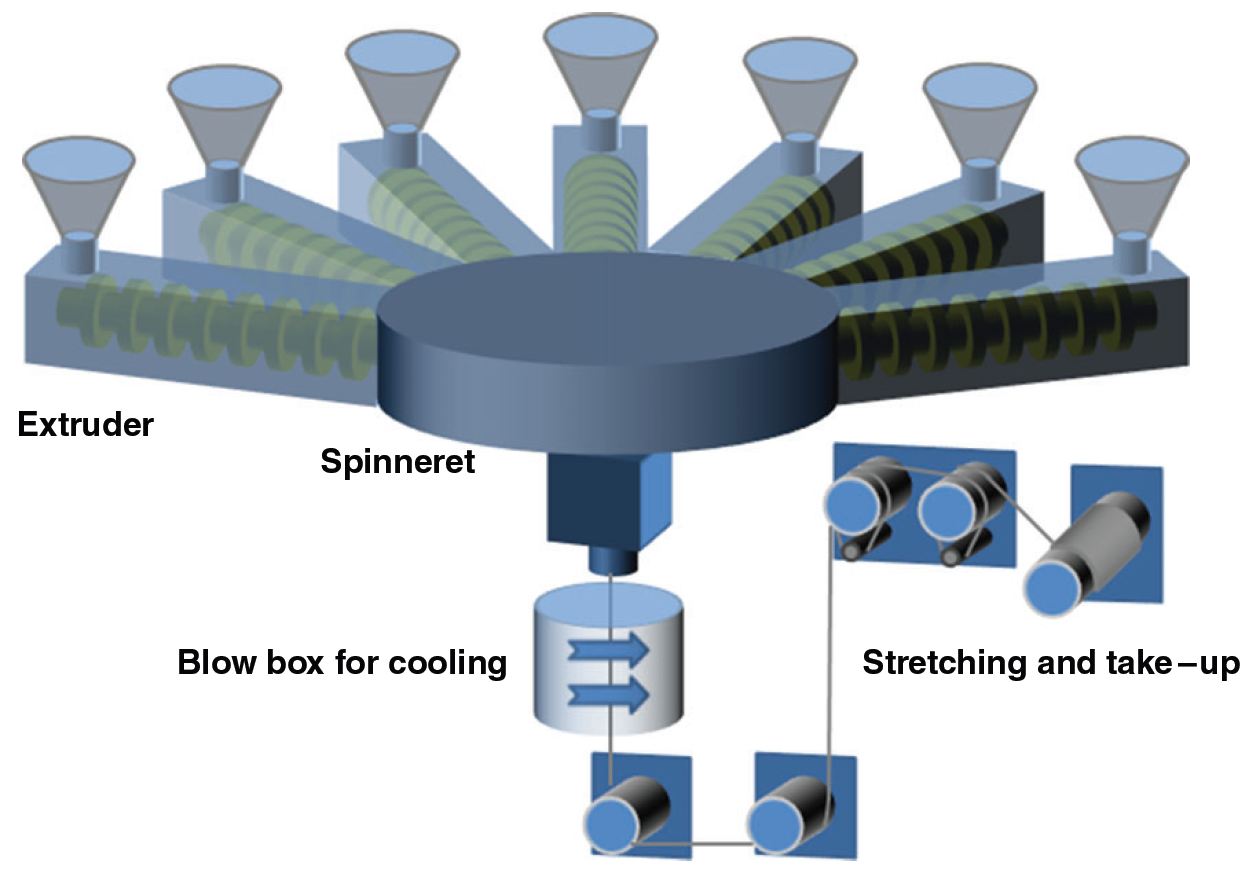
\includegraphics[height=0.25\textheight]{Bilder/Optische_Wellenleiter_Die_Polymer_Optische_Faser/Herstellung/pofmsispinn.png}
                \caption[kontinuirliche Extrusion einer polymer optischen Faser mit \textit{Multi Step Index} \newline \url{http://www.researchgate.net/publication/265646639_An_overview_on_fabrication_methods_for_polymer_optical_fibers} S. 5 (zuletzt aufgerufen am 28.09.2015)]{kontinuirliche Extrusion einer polymer optischen Faser mit \textit{Multi Step Index}}
                \label{fig:pofmsispinn}
            \end{center}
        \end{minipage}
    \end{center}
\end{figure}

\subsubsection{Herstellung einer GI-POF mittels eines modifizierten Schmelzspinnprozesses}

Ein weiteres Herstellungsverfahren ist ein modifizierter Schmelzspinnprozess der
RWTH Aachen. Dieses Verfahren eignet sich für die Herstellung von polymer
optischen Fasern mit Gradientenindexprofil. \autoref{fig:pofgispinn} zeigt die
Produktionsanlage bestehend aus einem Einfülltrichter (\textit{hopper}) für das
granulierte Kernmaterial und einem Extruder, welcher das Granulat erhitzt und in
die Spinndüse (\textit{spinning nozzle}) drückt. Die Spinndüse wandelt die
erhitzte Kernmaterialmasse zu einem Faden um. Dieser wird durch das Wasserbad
(\textit{water quench}) gezogen. Dabei ist der Abkühlungsvorgang für die
Enstehung des Gradientenindexprofils verantwortlich. Die von außen nach innen
abnehmende Kühlung führt zu unterschiedlichen Dichten und damit auch zu
unterschiedlichen Brechzahlen. In der letzten Einheit wird der Polymerfaden
gedehnt und aufgewickelt. Die Vorteile dieses Verfahrens liegen zum einen in der
ununterbrochenen Produktion des Wellenleiters und der damit verbundenen
Wirtschaftlichkeit und zum anderen in der Möglichkeit die Brechzahlen durch
Variierung der Wassertemperatur und der Verweilzeit des Fadens im Wasser zu
beeinflussen. \cite{pofspinn}

\begin{figure}[h]
    \begin{center}
        \begin{minipage}[t]{\textwidth}
            \begin{center}
                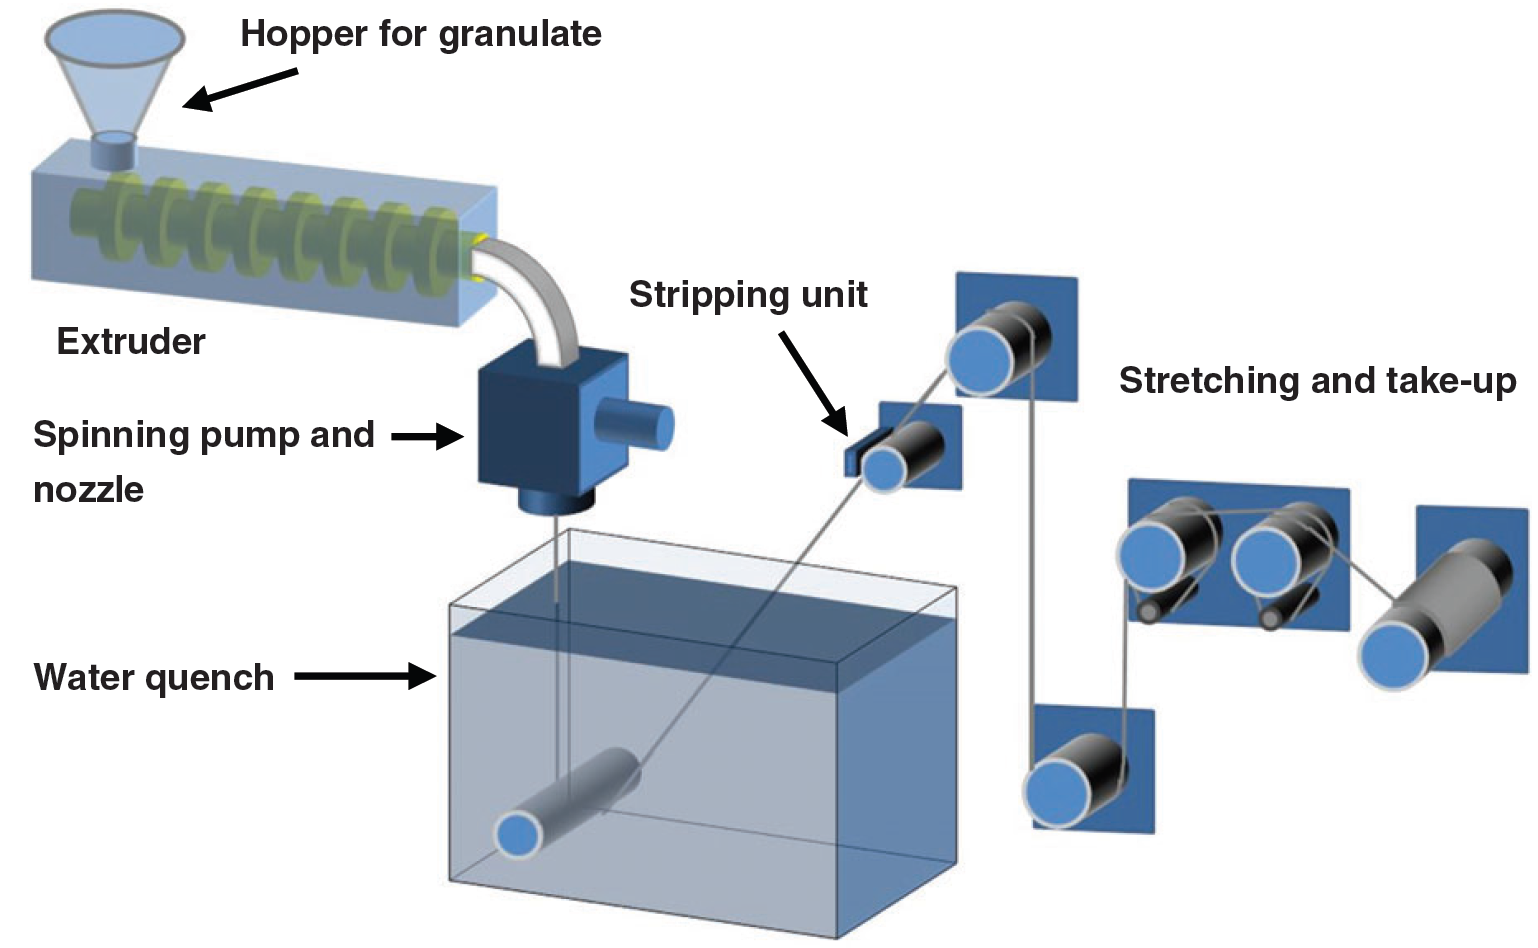
\includegraphics[height=0.25\textheight]{Bilder/Optische_Wellenleiter_Die_Polymer_Optische_Faser/Herstellung/pofgispinn.png}
                \caption[Schmelzspinnprozess zur Herstellung einer GI-POF \newline \url{http://www.researchgate.net/publication/265646639_An_overview_on_fabrication_methods_for_polymer_optical_fibers} S. 9 (zuletzt aufgerufen am 28.09.2015)]{Schmelzspinnprozess zur Herstellung einer GI-POF}
                \label{fig:pofgispinn}
            \end{center}
        \end{minipage}
    \end{center}
\end{figure}
